% Heutige Verwendung, Größe des Netzwerks, auch Contra-Argumente: Nutzung durch Kriminelle etc., Referenzierungen des Papers
%-Ein praktikables System
%-we feel that we must build a
%reputation for privacy, human rights, research, and other socially
%laudable activities. (Zitat aus unserem Paper Seite 14 links oben irgendwo)
%-Quelle: Internet (bei Berichten aus Krisenregionen, wie Kayro, Syrien), wenn es aus %em Darknet kommt.
%-Aktivisten können Anonym Bericht erstatten.
%-Kriminelle nutzen es auch (Zitat: Seite 14 oben links: Even though having more users would
%bolster our anonymity sets, we are not eager to attract the
%Kazaa or warez communities)


% also consider chapter 8
% current numbers (https://metrics.torproject.org/)

\section{Importance and impact}
A wide area network was briefly deployed after the invention of onion routing but it was not really used because it required a seperate "application proxy" for each supported application protocol and most of them were never written. Tor on the other hand uses the standard and near-ubiquitous SOCKS proxy interface, which supports most TCP-based programs without modification.

\begin{figure}
	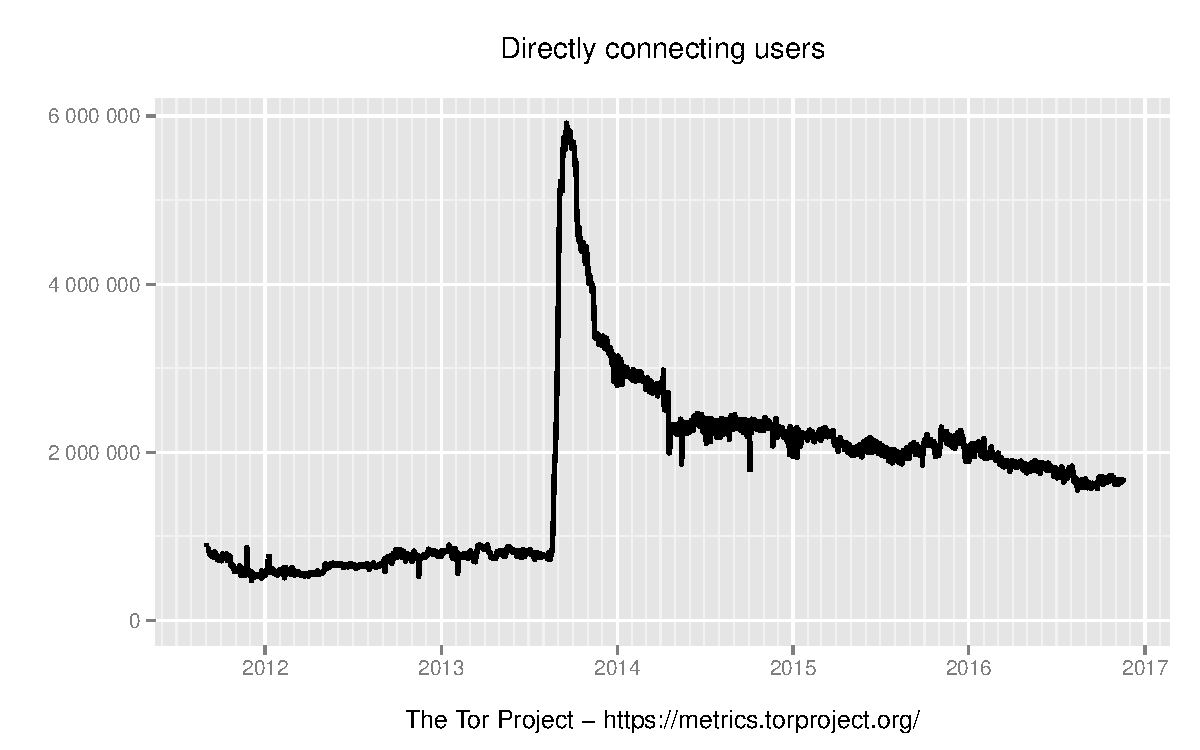
\includegraphics[width=\columnwidth]{img/userstats.pdf}
	\caption{Estimated number of users connecting to Tor. Taken from \cite{tormetrics}.}
	\label{img_userstats}
\end{figure}

Because of that Tor is used in the world wide web since 2004 for anonymous connections. Individuals use Tor for censorship circumvention to reach othervise blocked content, to keep websites from tracking them or their family members, to publish services without needing to reveal the location of them or for sensitive communication. Tor is also used by companies or Journalists to communicate with activists or whistleblowers\cite{tor}. Currently there are about two million people using Tor as figure \ref{img_userstats} states. The peak in August if 2013 was probably caused by a botnet using Tor for the communication between the bots and the command and control server\cite{torblog_botnet}. This is an example for the downside of enabling anonymous connections. Tor can also be used by criminals to sell drugs, child porn, weapons or other illegal things.   

Apart from the practical impact of the Tor network the published paper also has a big impact on computer science and was cited more than 3000 times by other papers dealing with improvements for or attacks against Tor, analysis of practical effects of the Tor network or using the developed approach to enable anonymous connections in other fields like VoIP systems.